\documentclass[UTF8, 12pt]{article}
% 中文支持
\usepackage[UTF8]{ctex}	
% pdf调用 封面
\usepackage{pdfpages}
% color宏包
\usepackage{color}  
% 导入图片
\usepackage{caption}
\usepackage{graphicx, subfig}
% 防止图片乱跑
\usepackage{float}
% 支持数学符号
\usepackage{amsmath}
% 支持代码块
\usepackage{listings}
% pdf加入大纲
\usepackage{hyperref}
% 大纲去红框
\hypersetup{hidelinks,
	colorlinks=true,
	allcolors=black,
	pdfstartview=Fit,
	breaklinks=true
}

% 绘制三线表
\usepackage{booktabs}    
% 消除警告
\usepackage{lmodern}

% 绘图
\usepackage{tikz}
\usetikzlibrary{positioning, shapes.geometric}
\tikzstyle{bag} = [align=center]

% 设置页面的环境,a4纸张大小,左右上下边距信息
\usepackage[a4paper, left=31.8mm, right=31.8mm, top=25.4mm, bottom=25.4mm]{geometry}

% 字体设置
\usepackage{fontspec}
\setmainfont{Times New Roman}

% 代码块的基本设置
\lstset{
 breaklines,%自动换行
 columns=fixed,       
 numbers=left,                                        % 在左侧显示行号
 numberstyle=\tiny\color{gray},                       % 设定行号格式
 frame=none,                                          % 不显示背景边框
 backgroundcolor=\color[RGB]{245,245,244},            % 设定背景颜色
 keywordstyle=\color[RGB]{40,40,255},                 % 设定关键字颜色
 numberstyle=\footnotesize\color{darkgray},           
 commentstyle=\it\color[RGB]{0,96,96},                % 设置代码注释的格式
 stringstyle=\rmfamily\slshape\color[RGB]{128,0,0},   % 设置字符串格式
 showstringspaces=false,                              % 不显示字符串中的空格
 language=python,                                        % 设置语言
}

% 两图片并排
% \begin{figure}[htbp]
% 	\centering
% 	\begin{minipage}{0.49\linewidth}
% 		\centering
% 		\includegraphics[width=0.9\linewidth]{figure/figure_1.jpg}
% 		\caption{title1}
% 		\label{label1} %文中引用该图片代号
% 	\end{minipage}
% 	%\qquad
% 	\begin{minipage}{0.49\linewidth}
% 		\centering
% 		\includegraphics[width=0.9\linewidth]{figure/figure_3.jpg}
% 		\caption{title2}
% 		\label{label2} %文中引用该图片代号
% 	\end{minipage}
% \end{figure}

% 导入图片
% \begin{figure}[H]
%     \centering % 居中 
%     % 图片文件的相对路径
%     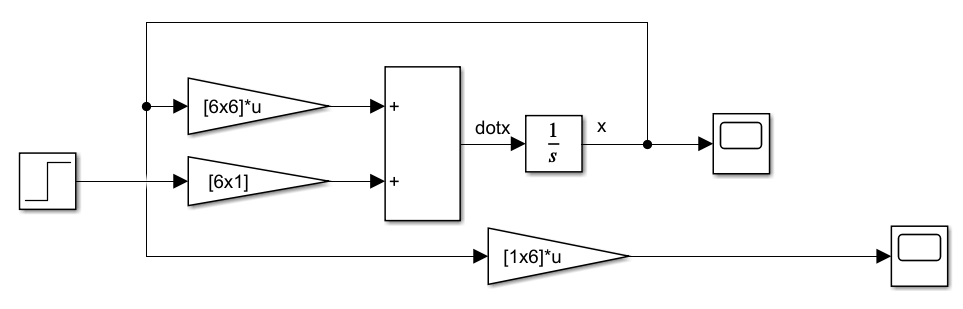
\includegraphics[width=.8\textwidth]{figure/exp1_1_model.png} 
%     \caption{Simulink模型} % caption是图片的标题
%     % \label{img} % 此处的label相当于一个图片的专属标志,目的是方便上下文的引用
% \end{figure}

% 导入代码
% \begin{lstlisting}
% a
% \end{lstlisting}

% 重置章节编号
% \setcounter{section}{0}

% \begin{table}[H] % 防止表格乱跑
% \centering % 居中
% \begin{tabular}{cccccc} % 指明列数
% 	\toprule % 顶部粗线
% 	序号 & 姓名 & 性别 & 年龄 & 身高/cm & 体重/kg \\
% 	\midrule % 中间细线
% 	1 & 张三 & M & 16 & 163 & 50 \\ % 每行末尾都要加换行符
% 	2 & 王红 & F & 15 & 159 & 47 \\
% 	3 & 李二 & M & 17 & 165 & 52 \\
% 	\bottomrule % 底部粗线
% \end{tabular}
% \caption{title} % 标题
% \end{table}

% \begin{thebibliography}{99}  
% 	\bibitem{ref1} 《现场总线技术及应用教程(第二版)》,王永华,机械工业出版社
%   \bibitem{ref13} \href{https://www.elecfans.com/kongzhijishu/1080520.html}{工业控制系统未来的发展趋势分析}:https://www.elecfans.com/kongzhijishu/1080520.html
% \end{thebibliography}


% 评分要点:工艺过程、现场需求、控制对象特性分析深入可靠;系统控制任务描述条理清楚,控制对象模型建立科学合理;传感器和执行机构选型、控制系统结构设计、控制器设计及其参数很好得满足系统性能、安全、可靠、经济性等要求;仿真实验假设合理,实验过程步骤详细,对比实验结果翔实可靠,考虑影响因素全面;对该系统工程设计中涉及的非技术性因素讨论深入。结课报告格式美观、逻辑清晰、结构合理、图表规范、语言流畅。控制系统设计过程中有自己独特思考或想法,具有一定的创新,并在报告中清晰完整地体现。

% 格式基本规范:报告正文字号为小四,中文采用宋体,英文采用 Times New Roman;段落首行缩进 2 字符,1.25 倍行间距,无段前段后间距。图表中的字体与正文一致,字号五号。报告中的各章节标题采用黑体,独立成行。
\begin{document}
% 小四字号
% \zihao{-4}
% \CJKfamily{song}

\begin{titlepage}
% 封面信息
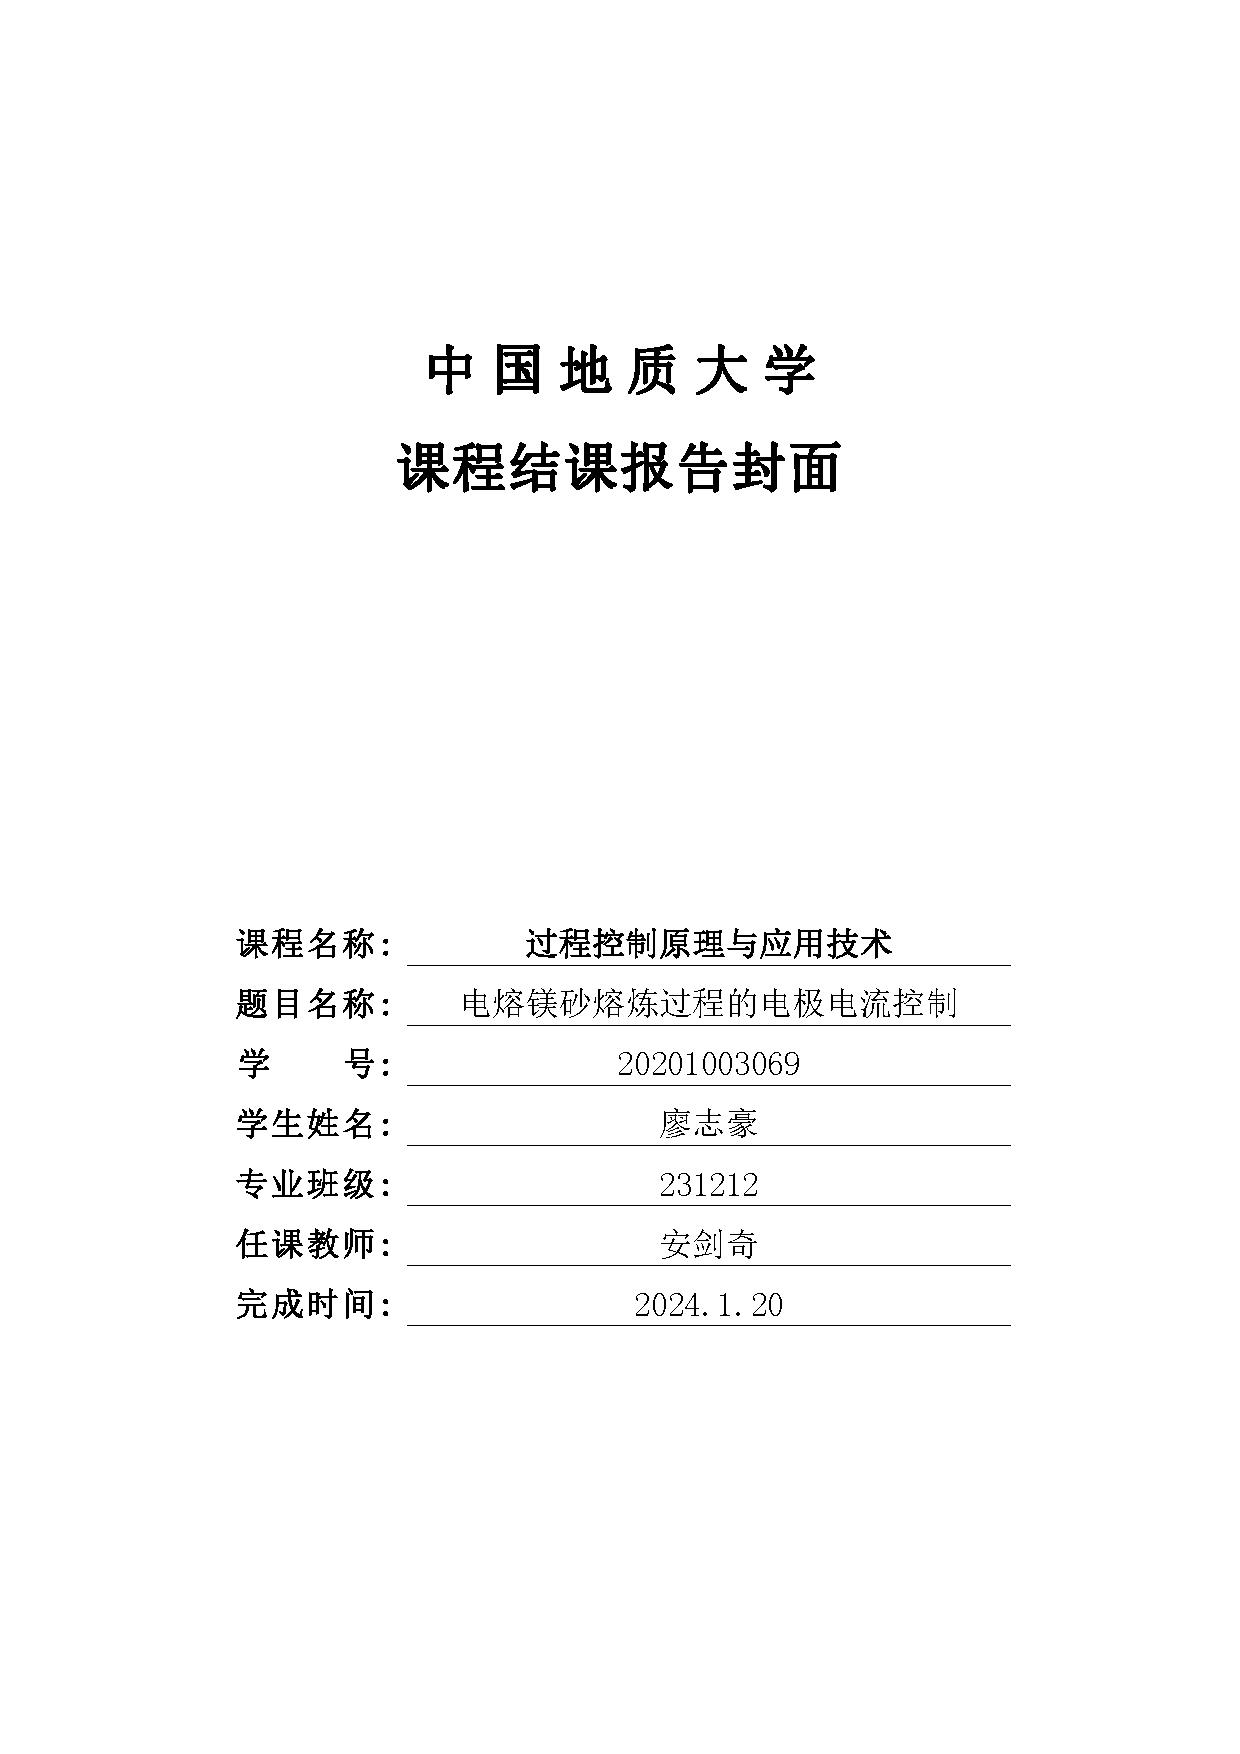
\includepdf[pages={1}]{./cover/cover.pdf}
\end{titlepage}

% 生成目录
\tableofcontents
\cleardoublepage

%
\section{内容介绍}
本文选取电熔镁砂熔炼过程作为过程控制案例,该案例以电熔镁炉为被控对象,以三相电极电流为被控量,交流电机转动的方向与频率作为控制量。在这一案例所涉及的工艺流程中,需要使得三相电极电流对给定值的跟踪误差在所有时间内均处于约束范围内,以保证工业生产的安全性,降低生产能耗和提高产品质量。

针对电熔镁砂熔炼过程中的电极电流控制问题,本文所参考的文献《电熔镁砂熔炼过程带输出补偿的PID控制》一文中设计了一种基于输出补偿的PID控制器,相较普通的PID控制算法,该方法可以在所有运行时间内将电流跟踪误差控制在目标范围内,取得了更好的控制效果。本文主要针对作者在该论文中所做的工作进行比较详细的学习和研究,并针对论文中的仿真实验进行了复现。

除此之外,在另一篇与之相关的文献《基于补偿控制的自适应模型预测控制》中,该论文作者应用所提出的基于补偿控制的自适应模型预测控制方法,同样对电熔镁砂熔炼过程中的电极电流控制问题进行了仿真实验。本文对该文献中涉及到的预测模型控制方法进行了学习和复现,并针对同一过程控制案例给出了相应的仿真实验结果。


% 本文对张雪敏等人在《基于补偿控制的自适应模型预测控制》一文中所做的工作进行学习和复现。

% 在该文章中,作者针对离散时间仿射非线性系统往往具有参数未知、外部干扰未知并且带有输入输出约束的特点,提出了一种基于补偿控制的自适应模型预测控制方法。该方法在传统MPC控制的基础上,利用基于高阶干扰观测器的投影算法对未知参数和外部干扰进行同步估计,并根据干扰观测值和参数估计值设计补偿控制量;结合补偿控制、参数估计等方法与传统MPC构成一种新型的基于补偿控制的自适应MPC控制系统结构。

% 本文首先对该文章中提出的基于补偿控制的自适应模型预测控制方法进行简要介绍、分析和补充,然后将该方法应用于一个工业过程控制案例,即电熔镁砂熔炼过程中的电极电流的控制问题,并给出相应的复现仿真结果。

% \textcolor{red}{对案例进行分析,理解和复现}

%
\section{研究背景与研究动机}

电熔镁砂是化工、航天等工业所需耐火材料的主要原料,其制造以菱镁矿石为原矿,采用埋弧方式进行熔炼。电熔镁砂熔炼过程中控制系统需要通过调整三相电极与熔池之间的距离,对各电极之间的电阻进行调节,进而控制三相电极电流跟踪熔化电流,使之产生电弧,并通过电弧放热使原矿受热熔化形成熔液,在熔化的同时不断加入原矿,当熔池升高到炉口上表面时熔炼结束,经冷却结晶后生成成品。

在上述工业过程中,电熔镁炉的耗能占整个工业生产的绝大部分。电熔镁炉作为一种典型的高耗能生产设备,其完成一炉原矿的熔炼大约需要40000千瓦时的耗电量,其电能成本占生产成本的60\%以上。

为了改善该工业生产过程中的高耗能,同时保证产品质量,需要对生产过程进行控制。一方面,要保证生产的产品具有足够的合格率,需要将电极电流控制在熔化电流范围内;在另一方面,要保证每吨产品的生产能耗尽可能小,需要将电极电流控制在最佳熔化电流附近。因此,针对电熔镁炉的电流控制具有非常重要的研究意义。



% 参数未知,外部干扰未知并且带有输入输出约束的离散时间仿射非线性系统,提出了一种基于补偿控制的自适应模型预测控制方法

% 针对电熔镁砂熔炼过程中的电极电流控制问题,进行仿真

%
\section{研究内容}

%%
\subsection{电熔镁砂熔炼过程中的电极电流控制}
% - 工艺过程分析
% 被控量
% 控制量
% 干扰量
% - 控制对象分析与建模
% - 带输出补偿的PID控制

% - 设计基于补偿控制的自适应模型预测控制系统


%%%
\subsubsection{电熔镁砂熔炼过程简介}
如下图所示,电熔镁炉熔炼系统由电流控制系统、三个交流电机和三根电极组成的电极移动系统、原矿仓和电振给料机组成的加料系统、供电系统和电熔镁炉构成。
\begin{figure}[H]
    \centering % 居中 
    % 图片文件的相对路径
    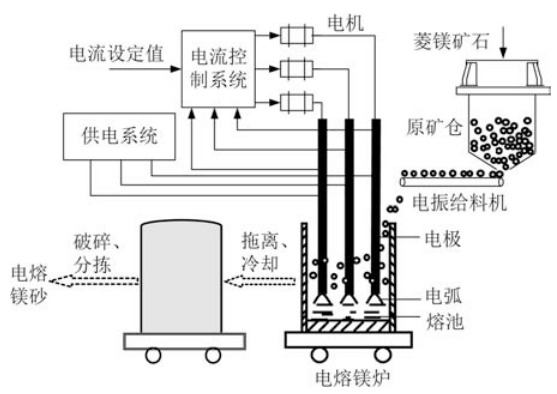
\includegraphics[width=.8\textwidth]{figure/电熔镁砂熔炼过程示意图.png} 
    \caption{电熔镁砂熔炼过程示意图} % caption是图片的标题
    % \label{fig:img} % 此处的label相当于一个图片的专属标志,目的是方便上下文的引用
    % 图片引用格式:\ref{fig:img} 可能需要二次编译
\end{figure}

熔炼过程首先由加料系统向炉内加入菱镁矿石,通过供电系统向三相电极供电,产生电弧。原矿吸收电弧放出的热量熔化,形成熔池。电流控制系统通
过电极移动系统调节电极与熔池之间的距离,进而控制阻抗使三相电极平均电流跟踪熔化电流设定值。由于熔化温度高,因此采用埋弧方式。三相电极埋在原矿之中,边熔化边加料,随着原矿的不断加入和熔化,熔池增高,当达到炉口上表面时,熔炼过程结束。使用小车将炉体拖离熔炼工位,进行自然冷却并破碎,得到电熔镁砂产品。

%%%
\subsubsection{工艺过程分析}

% - 结构 
% - 执行器
% - 控制器 正反作用

% 被控对象:电熔镁炉
% 被控量:三相电极的电流
% 控制量:电极与熔池之间的距离,交流电机转动方向与频率
% 执行器:交流电机

通过分析可以知道,在上述电熔镁砂熔炼工艺过程中,电熔镁炉作为被控对象,炉中的三相电极之间的平均电流作为系统的被控量,其大小是否合适决定了该工业过程的产品质量以及生产能耗。系统的控制量为三个交流电机的转动方向和频率,在后续对控制对象进行建模时该控制量以单个变量来表示,作为系统的输入;同时交流电机也作为该系统的执行器来调节三相电极的位置,以控制电极与熔池之间的距离。系统运行过程中,为了对三相电极之间的平均电流进行检测和监视,需要设置相应的电流检测变送装置,并将检测信号传送至电流控制系统。电流控制系统在此处主要充当控制器的角色,其控制算法主要基于PID控制策略。

此外,通过上面展示的电熔镁砂熔炼过程示意图不难看出,原矿仓和电振给料机的给料速度也会对熔炼过程造成影响。另外,电熔镁砂的熔炼过程通常会受到杂质成分、工况条件等不确定性因素以及外部不可测扰动的影响,这些都可以看作控制过程中的干扰量。


%%%
\subsubsection{控制对象特性分析与建模}

%%%%
\paragraph{执行器与控制器特性分析}~{}

电熔镁砂熔炼系统使用交流电机作为控制系统中的执行器部分。对于此处所用的交流电机,我们可以指定它们的转动方向和工作频率,以决定三相电极的升降方向和移动速度。由于作者在文中并未对此做详细介绍,此处为方便讨论,不妨假设当交流电机输入信号$u$为正值时,电机转动方向为正,三相电极向上移动;反之,当输入信号$u$为负值时,电机转动方向为负,三相电极向下移动;且输入信号绝对值越大,则电机转速越高,对应三相电极的移动速度越快。

基于以上假设,经过分析可以知道,由于当执行器输入信号越大时,三相电极向上移动越多,导致三相电极之间的阻抗越大,进而导致电熔镁炉中三相电极之间的平均电流变小,即被控量减小。因此,此处如果将控制系统中的执行器、被控对象和被控过程、检测变送环节等视为一个广义被控对象,则不难发现该广义被控过程是一个反作用过程,即输入值越大,输出值越小,其放大系数为负。进而如果以单回路控制系统为例对该控制案例进行分析,则控制系统的控制部分应当是一个正作用控制器,其放大系数为负值。

%%%%
\paragraph{控制对象模型建立}~{}

电熔镁砂熔炼过程的模型构建比较繁琐,模型建立的细节可以参考文献相关部分,此处不再赘述。基于文中的模型建立方法,可以得到如下的三相电极电流动态模型:
\begin{equation*}
	\frac{d y_i(t)}{dt} = -\frac{\sqrt{3}y_i^2(t)}{U} \cdot \{ \frac{f_1(\cdot)}{\pi r_{iarc}^2}[\frac{2\pi(1-s)u_i(t)}{p}r_d - \dot{h}_{ipool}(\cdot)] + \frac{f_2(\cdot)}{2\pi h_{ipool}^2(\cdot)}\dot{h}_{ipool}(\cdot) \}
\end{equation*}

该式表明电流动态模型具有强非线性,模型参数$f_1(\cdot),\ f_2(\cdot),\ h_{ipool},\ \dot{h}_{ipool}$为随熔炼过程和原矿颗粒长度及杂志成分的变化而变化的非线性函数。将上述电极电流被控对象模型进一步简化得到:
\begin{equation*}
	\dot{y}_i(t) = \frac{\sqrt{3}}{\pi}F_i(\cdot)y^2_i(t) - 2\sqrt{3}Q_i(\cdot)u_i(t)y_i^2(t)
\end{equation*}

其中$F_i(\cdot),\ Q_i(\cdot)$为电流模型的非线性部分简化后参数,且有:
\begin{align*}
	F_i(\cdot) &= [\frac{f_1(\cdot)}{r_{iarc}^2} - \frac{f_2(\cdot)}{2h_{ipool}^2}(\cdot)] \frac{\dot{h}_{ipool}(\cdot)}{U} \\
	Q_i(\cdot) &= \frac{f_1(\cdot)(1-s)r_d}{Ur_{iarc}^2p} 
\end{align*}

采用欧拉法将上述电极电流动态模型式离散化,同时将上述非线性部分简化后参数作为待辨识参数,于是电极电流仿真模型如下:
\begin{equation*}
	y_i(k+1) = y_i(k) + \delta_t \frac{\sqrt{3}}{\pi}\hat{F}_iy_i^2(k) - \delta_t2\sqrt{3}\hat{Q}_iu_i(k)y_i^2(k) + \delta \hat{y}_i(k)
\end{equation*}

其中,$\delta_t$为采样时间。

%%
\subsection{带输出补偿的PID控制方法}
%%%
\subsubsection{带输出补偿的PID控制算法原理简介}
带输出补偿的PID控制系统结构图如下所示:
\begin{figure}[H]
    \centering % 居中 
    % 图片文件的相对路径
    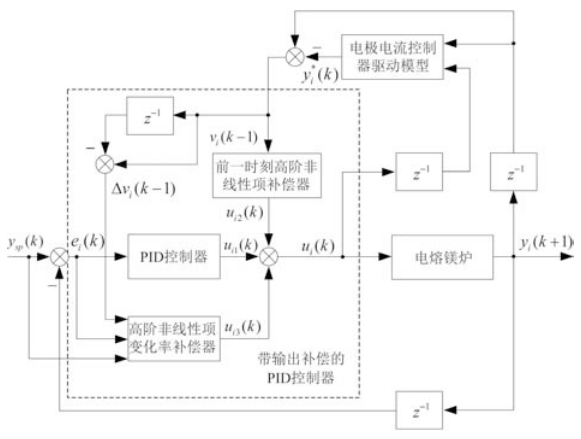
\includegraphics[width=.8\textwidth]{figure/带输出补偿的PID控制结构框图.png} 
    \caption{带输出补偿的PID控制结构框图} % caption是图片的标题
    % \label{img} % 此处的label相当于一个图片的专属标志,目的是方便上下文的引用
\end{figure}

% - 控制策略
% - 控制器设计

带输出补偿的PID控制律为:
\begin{equation*}
	u_i(k) = u_{i1}(k) + u_{i2}(k) + u_{i3}(k)
\end{equation*}

其中,$u_{i1}(k)$为针对系统的确定线性部分模型设计的控制率,由如下公式确定:
\begin{align*}
	& H_i(z^{-1})u_{i1}(k) = G_i(z^{-1})e_i(k) \\
	& e_i(k) = y_{sp}(k) - y_i(k) \\
	& H_i(z^{-1}) = 1 - z^{-1} \\
	& G_i(z^{-1}) = g_{i0} + g_{i1}z^{-1} + g_{i2}z^{-2}
\end{align*}

$g_{i0},\ g_{i1},\ g_{i2}$为PID控制器参数,$e_i(k)$为跟踪误差。为方便计算,可以将上式化为:
\begin{equation*}
	u_{i1}(k) = u_{i1}(k-1) + g_{i0}e_i(k) + g_{i1}e_i(k-1) + g_{i2}e_i(k-2) 
\end{equation*}

前一时刻高阶非线性项$v_i(k-1)$补偿器为:
\begin{equation*}
	u_{i2}(k) = -K_i(z^{-1})v_i(k-1)
\end{equation*}

其中$K_i(z^{-1})$为补偿器的参数。作者在文中采用一步最优前馈控制律,对$K_i(z^{-1})$中的参数进行设计,以实现对$v_i(k-1)$的动态和静态补偿。其确定公式如下:
\begin{equation*}
	K_i(z^{-1}) = \frac{1}{B_i(z^{-1})} = k_{vi0}
\end{equation*}

高阶非线性项变化率补偿器为:
\begin{align*}
	u_{i3}(k) &= \frac{1}{H_i(z^{-1})B_i(z^{-1})}G'_i(z^{-1})e_i(k) - \\
	& \frac{1}{B_i(z^{-1})}\Delta v_i(k-1) + \frac{A_i(z^{-1})}{B_i(z^{-1})}y_{sp}(k+1)
\end{align*}

其中,高阶非线性项变化率补偿器参数可由下式计算得到:
\begin{align*}
	G'_i(z^{-1}) &= A_i(z^{-1}) - B_i(z^{-1})G_i(z^{-1}) - a_{i1} \\
	&= (1 - b_{i0}g_{i0} - a_{i1}) + (a_{i1} - b_{i0}g_{i1})z^{-1} - b_{i0}g_{i2}z^{-2} \\
	&= g'_{i0} + g'_{i1}z^{-1} + g'_{i2}z^{-2}
\end{align*}

%%%
\subsubsection{带输出补偿的PID控制算法实现步骤}
\begin{enumerate}
	\item 对于电极电流模型:
	\begin{equation*}
		A_i(z^{-1})y_i(k+1) = B_i(z^{-1})u_i(k) + v_i(k-1) + \Delta v_i(k)
	\end{equation*}
	\begin{equation*}
		A_i(z^{-1}) = 1 + a_{i1}z^{-1},\ B_i(z^{-1}) = b_{i0}
	\end{equation*}
	采用实际熔炼过程输入输出数据,利用递推最小二乘和神经网络交替辨识其中的参数$a_{i1}$和$b_{i0}$;
	
	\item 由文中式(37)确定PID控制器参数$g_{i0}$、$g_{i1}$和$g_{i2}$:
	\begin{equation*}
		A_i(z^{-1})H_i(z^{-1}) + z^{-1}B_i(z^{-1})G_i(z^{-1}) \ne 0,\ |z| > 1
	\end{equation*}
	
	\item 由下式确定前一时刻高阶非线性项$v_i(k-1)$补偿器参数$k_{vi0}$:
	\begin{equation*}
		K_i(z^{-1}) = \frac{1}{B_i(z^{-1})} = k_{vi0}
	\end{equation*}

	\item  由下式确定前一时刻高阶非线性项变化率$\Delta v_i(k)$补偿器参数$g'_{i0},\ g'_{i1},\ g'_{i2}$:
	\begin{align*}
		G'_i(z^{-1}) &= A_i(z^{-1}) - B_i(z^{-1})G_i(z^{-1}) - a_{i1} \\
		&= g'_{i0} + g'_{i1}z^{-1} + g'_{i2}z^{-2}
	\end{align*}

	\item 采集输入输出数据, 求出跟踪误差$e_i(k)$,并由下式求出前一时刻高阶非线性项$v_i(k-1)$:
	\begin{align*}
		v_i(k-1) &= y_i(k) + A^*_i(z^{-1})y_i(k) - B_i(z^{-1})u_i(k-1) \\
		&= y_i(k) - y^*_i(k) \\
		A^*_i(z^{-1}) &= a_{i1}z^{-1}
	\end{align*}
	$y^*_i(k) = -a_{i1}y_i(k-1) + b_{i0}u_i(k-1)$为电极电流控制器驱动模型。

	由下式求出前一时刻高阶非线性项变化率$\Delta v_i(k-1)$:
	\begin{equation*}
		v_i(k) = v_i(k-1) + \Delta v_i(k)
	\end{equation*}

	\item 由下式求出PID控制器输出$u_{i1}(k)$:
	\begin{equation*}
		H_i(z^{-1})u_{i1}(k) = G_i(z^{-1})e_i(k)
	\end{equation*}
	
	由下式求出前一时刻高阶非线性项补偿器输出$u_{i2}(k)$:
	\begin{equation*}
		u_{i2}(k) = -K_i(z^{-1})v_i(k-1)
	\end{equation*}
	
	由下式求出前一时刻高阶非线性项变化率补偿器输出$u_{i3}(k)$:
	\begin{align*}
		u_{i3}(k) &= \frac{1}{H_i(z^{-1})B_i(z^{-1})}G'_i(z^{-1})e_i(k)  \\
		& - \frac{1}{B_i(z^{-1})}\Delta v_i(k-1) + \frac{A_i(z^{-1})}{B_i(z^{-1})}y_{sp}(k+1)
	\end{align*}
	为方便计算,可以改写为:
	\begin{align*}
		u_{i3}(k) &= u_{i3}(k-1) + \frac{1}{b_{i0}}[g'_{i0}e_i(k) + g'_{i1}e_i(k-1) + g'_{i2}e_i(k-2) \\
		& + \Delta v_i(k-1) - \Delta v_i(k-2) \\
		& + y_{sp}(k+1) + (a_{i1} - 1)y_{sp}(k) - a_{i1}y_{sp}(k-1)]
	\end{align*}

	\item 由下式求出带输出补偿的PID控制器输出$u_i(k)$,加到电熔镁炉被控对象上:
	\begin{equation*}
		u_i(k) = u_{i1}(k) + u_{i2}(k) + u_{i3}(k)
	\end{equation*}

	\item $t = k+1$,返回步骤5。
\end{enumerate}


%%
\subsection{基于补偿控制的自适应模型预测控制系统设计}
% - 研究对象
% - 基于高阶观测器的投影算法
% - 补偿控制 MPC优化问题
% - 基于补偿控制的自适应MPC算法设计步骤

基于补偿控制的自适应MPC控制系统结构图如下所示(摘录自原文):
\begin{figure}[H]
    \centering % 居中 
    % 图片文件的相对路径
    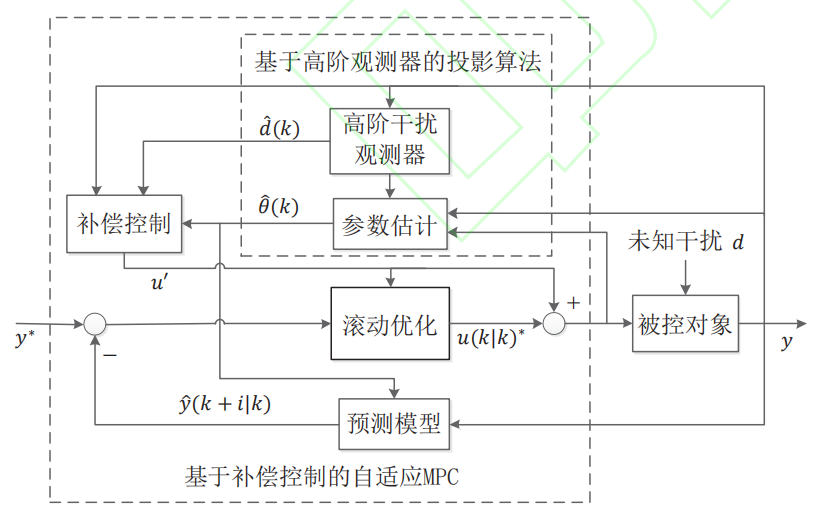
\includegraphics[width=.8\textwidth]{figure/基于补偿控制的自适应MPC系统结构.png} 
    \caption{基于补偿控制的自适应MPC系统结构} % caption是图片的标题
    % \label{img} % 此处的label相当于一个图片的专属标志,目的是方便上下文的引用
\end{figure}
下面将根据文献内容对该系统做简要介绍。

%%%
\subsubsection{研究对象}
选取一阶离散时间仿射非线性系统作为研究对象,其差分方程数学模型一般可以表示为:
\begin{equation*}
	y(k+1) = y(k) + af(y(k)) + bg(y(k))u(k) + d(k) + \Delta y(k)
\end{equation*}
其中,$d(k)$表示未知外部干扰项。算子$\Delta$表示一阶差分操作,$\Delta y(k)$是差分方程建模的误差补偿项,且有:
\begin{equation*}
	\Delta y(k) = y(k) - y(k-1)
\end{equation*}
同时系统的输入$u(k)$与输出$y(t)$需要满足如下约束:
\begin{equation*}
	\begin{cases}
		u_{min} < u(k) < u_{max} \\
		y_{min} < y(k) < y_{max} \\
	\end{cases}
\end{equation*}

%%%
\subsubsection{基于高阶观测器的投影算法}
为了对工业过程中的未知参数以及干扰进行估计,作者引入了基于高阶观测器的投影算法。该方法实质上是一种结合了高阶观测器和投影算法的参数辨识算法。

基于高阶观测器的投影算法如下:
\begin{equation*}
	\hat{\theta}(k) = \hat{\theta}(k-1) + \frac{s(k-1)\hat{\varphi}(k-1)}{c + \hat{\varphi}(k-1)^T\hat{\varphi}(k-1)} e(k)
\end{equation*}
\begin{equation*}
	s(k-1) = 
	\begin{cases}
		1,\quad |e(k)| > 2D \\
		0,\quad 其他
	\end{cases}
\end{equation*}
\begin{align*}
	\hat{d}(k) &= \hat{d}(k-1) + L_0[y(k) - \hat{y}(k)] + \Delta\hat{d}(k-1) + \\
	&= L_1[\Delta y(k) - \Delta\hat{y}(k)] + ... + \Delta^{\eta}\hat{d}(k-1) + \\
	&= L_{\eta}[\Delta^{\eta}y(k) - \Delta^{\eta}\hat{y}(k)]
\end{align*}
\begin{equation*}
	\hat{y}(k) = 2y(k-1) - y(k-2) + \hat{\varphi}(k-1)^T\hat{\theta}(k-1)
\end{equation*}

其中,$\hat{\theta}(k)$为$k$时刻参数向量的估计;$c \in R,\ c > 0$;$e(k)$为$k$时刻系统的估计误差。

%%%
\subsubsection{补偿控制与MPC优化问题}
%%%%
\paragraph{补偿控制}~{}

参数估计误差和未知干扰的存在会给MPC优化问题的求解带来局限,针对这一问题,文章中设计了补偿控制方法。求解补偿控制量$u'$的公式如下:
\begin{equation*}
	[\hat{b}(k) + \beta]g(y(k))u' + \hat{d}(k) + D + \gamma f(y(k)) + \beta g(y(k))u_{max} = 0
\end{equation*}

其中$u_{max}$为输入约束给定的上界。

%%%%
\paragraph{MPC优化问题}~{}

MPC优化问题的核心是,基于系统当前的输出和设定值,找到未来一段时间内的一组控制信号$U^*$,使得系统在这段时间内的输出尽可能符合预期的变化情况,即参考轨迹。对于所得到的一组最优控制序列,选择其中的第一个元素与补偿控制量$u'$相加作为当前的控制信号。

对于参考轨迹的获取,作者在文章中并未给出具体的方法。这里我结合老师在课程中讲授的预测模型控制算法,查阅有关资料后得到了一种常用的设计方法。

参考轨迹通常采用一阶指数曲线形式。设过程输出的设定值为$y_d$,参考轨迹为$y_r$,以当前时刻(第$k$时刻)的系统实际输出作为起始值,则$y_r$在未来若干时刻的值可以通过如下公式计算得到:
\begin{equation*}
	\begin{cases}
		y_r(k) = y(k) \\
		y_r(k + i) = \alpha^iy(k) + (1 - \alpha^i)y_d,\quad i = 1,2,...,P
	\end{cases}
\end{equation*}

式中,$\alpha = e^{-T/T_r}$,$T$为采样周期,$T_r$为参考轨迹的时间常数。$\alpha$是参考轨迹的重要设计参数,$\alpha$越大,参考轨迹越平滑,鲁棒性越强,但控制的快速性会变差。

文中所构建的MPC优化问题表示如下:
\begin{equation*}
	\min\sum_{i=1}^{N_p} \{ s\cdot[\hat{y}(k+i|k) - y^*(k+1)]^2 + r\cdot u(k+i|k)^2 \}
\end{equation*}
$s.t.$
\begin{equation*}
	\hat{y}(k+1|k) = y(k|k) + \hat{a}(k)f(y(k|k)) + \hat{b}(k)g(y(k|k))u(k) + \Delta y(k|k)
\end{equation*}
\begin{align*}
	\hat{y}(k+i|k) &= \hat{y}(k+i-1|k) + \hat{a}(k) f(\hat{y}(k+i-1|k)) + \\
	& \hat{b}(k)g(\hat{y}(k+i-1|k))u(k+i-1|k) + \Delta\hat{y}(k+i-1|k)
\end{align*}
\begin{equation*}
	i = 2,...,N_p
\end{equation*}
\begin{equation*}
	y_{min} < \hat{y}(k+i|k) < y_{max},\quad i = 1, ..., N_p
\end{equation*}
\begin{equation*}
	u_{min} - u' < u(k) < u_{max} - u'
\end{equation*}
\begin{equation*}
	u_{min} < u(k+i|k) < u_{max},\quad i = 1, ..., N_c - 1
\end{equation*}

%%%
\subsubsection{基于补偿控制的自适应MPC算法设计步骤}
基于补偿控制的自适应MPC算法设计步骤如下:
\begin{enumerate}
	\item 置初值$\hat{\theta}(0)$;
	
	\item 在$k$时刻通过基于干扰观测器的投影算	法同步辨识得到干扰观测值$\hat{d}(k)$和参数估计	值$\hat{\theta}(k)$。
	
	\item 根据下式计算补偿控制量$u'$:
	\begin{equation*}
		[\hat{b}(k) + \beta]g(y(k))u' + \hat{d}(k) + D  + \gamma f(y(k)) + \beta g(y(k))u_{max} = 0
	\end{equation*}

	\item 求解MPC优化问题得到解$u^∗(k|k)$,将控制律$u(k) = u^∗(k|k) + u'$作用于系统:
	\begin{equation*}
		y(k+1) = y(k) + af(y(k)) + bg(y(k))u(k) + d(k) + \Delta y(k)
	\end{equation*}	
\end{enumerate}


%
\section{结果复现}
% - 数值仿真
% - 针对电熔镁砂熔炼过程中的电极电流控制问题仿真

% - 搭建simulink模型

%%
\subsection{基于带输出补偿的PID控制算法的仿真验证}
%%%
\subsubsection{被控对象仿真模型}
经前述分析可以得到电极电流被控对象的动态模型表示:
\begin{equation*}
	\dot{y}_i(t) = \frac{\sqrt{3}}{\pi}F_i(\cdot)y^2_i(t) - 2\sqrt{3}Q_i(\cdot)u_i(t)y_i^2(t)
\end{equation*}

其中$F_i(\cdot),\ Q_i(\cdot)$为电流模型的简化后参数,采用参数辨识方法对其进行离线辨识,此处可以忽略它们的表达式。

采用欧拉法将上述电极电流动态模型式离散化,使用实际工业过程中大量的电极电流和电机转动方向与频率数据,采用递推最小二乘和神经网络交替辨识方法对电流模型的参数$F_i(\cdot),\ Q_i(\cdot)$及建模误差$\Delta y_i(k)$进行辨识。此外,在仿真过程中还需要考虑随机噪声干扰的影响,于是电极电流仿真模型如下:
\begin{equation*}
	y_i(k+1) = y_i(k) + \delta_t \frac{\sqrt{3}}{\pi}\hat{F}_iy_i^2(k) - \delta_t2\sqrt{3}\hat{Q}_iu_i(k)y_i^2(k) + \Delta \hat{y}_i(k) + noise(k)
\end{equation*}

其中,$\delta_t$为采样时间,$noise(k)$为随机噪声序列。按照文中的描述,此处的$\hat{F}_i,\ \hat{Q}_i,\ \Delta \hat{y}_i(k)$需要预先通过辨识得到。

%%%
\subsubsection{控制器参数设定}
%%%%
\paragraph{控制目标}~{}

根据实际电熔镁砂熔炼过程中的工艺要求,即需要在所有运行时间内将熔炼过程的三相电极电流平均值$y(k)$与设定值$y_{sp}(k)$的跟踪误差$e(k)$控制在给定目标范围内,则控制目标可以表示为:
\begin{equation*}
	|e(k)| = | y_{sp}(k) - y(k) | < 2000,\ 0 < k < \infty
\end{equation*}

考虑到生产安全等因素,还需要对交流电机转速和电极电流等过程量做一些约束。此处给出设定值$y_{sp}(k) = 14500A$,且存在如下约束条件:
\begin{equation*}
	12000 < y_1(k) < 17000
\end{equation*}
\begin{equation*}
	-20 < u_1(k) < 20
\end{equation*}

%%%%
\paragraph{控制器参数设定}~{}

根据作者在文中所给仿真参数,此处将电极电流控制器参数设置为:
\begin{align*}
	A_1(z^{-1}) &= 1 - 1.0019z^{-1} \\
	B_1(z^{-1}) &= 0.454
\end{align*}

因而可以通过计算得到带输出补偿的PID控制器参数设定:
\begin{align*}
	G_1(z^{-1}) &= -1.295 + 1.82z^{-1} - 0.56z^{-2} \\
	K_1(z^{-1}) &= -2.2026 \\
	G'_1(z^{-1}) &= 1.414 - 0.1756z^{-1} - 0.2542z^{-2}
\end{align*}

此外,设计一个常规控制器用于进行对比分析,其参数设定与$G_1(z^{-1})$相同。

%%%
\subsubsection{仿真结果和分析}
% - 基于输出补偿PID控制的结果 输入输出
% - 常规PID控制结果
采用递推最小二乘和神经网络算法对系统模型参数进行辨识,得到$F_1(\cdot)$,$Q_1(\cdot)$的估计值分为:
\begin{equation*}
	\hat{F}_1 = -1.344 ,\ \hat{Q}_1 = 7.059 \times 10^{-4}
\end{equation*}

仿真过程中所用的噪声信号为$[-500, 500]$范围内的随机噪声,如下图所示:
\begin{figure}[H]
    \centering % 居中 
    % 图片文件的相对路径
    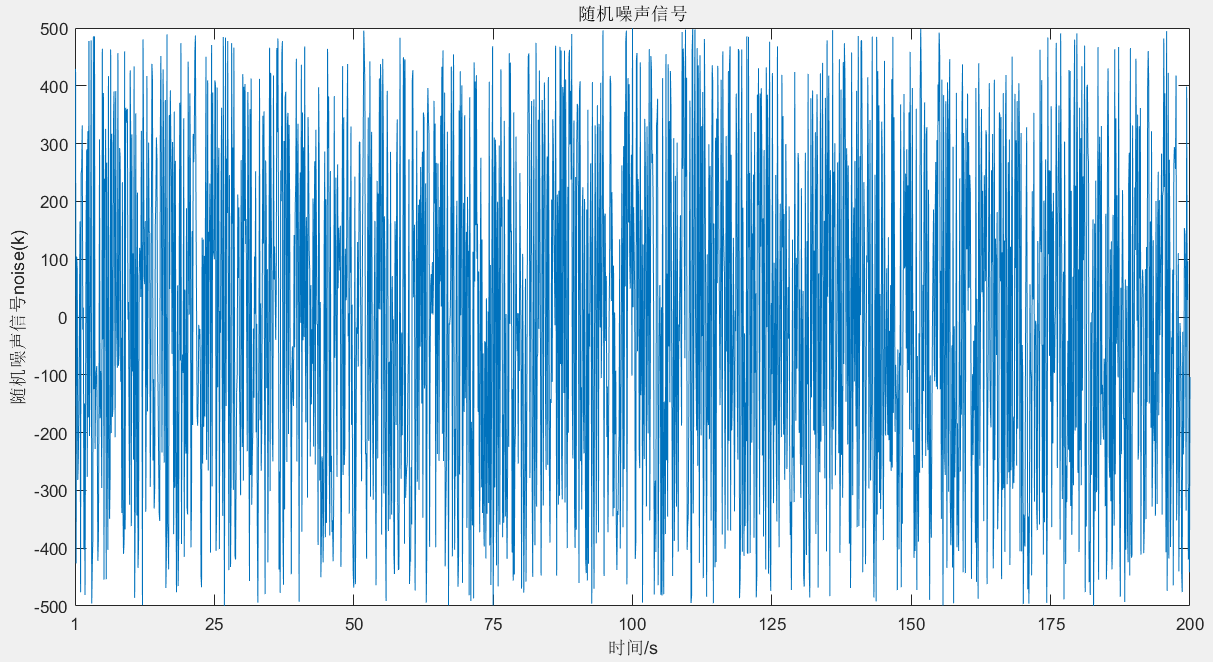
\includegraphics[width=.8\textwidth]{figure/随机噪声信号.png} 
    \caption{随机噪声信号} % caption是图片的标题
    % \label{fig:img} % 此处的label相当于一个图片的专属标志,目的是方便上下文的引用
    % 图片引用格式:\ref{fig:img} 可能需要二次编译
\end{figure}

分别使用基于输出补偿的PID控制器和常规控制器对电极电流进行控制,仿真对比实验结果如下所示:
\begin{figure}[H]
    \centering % 居中 
    % 图片文件的相对路径
    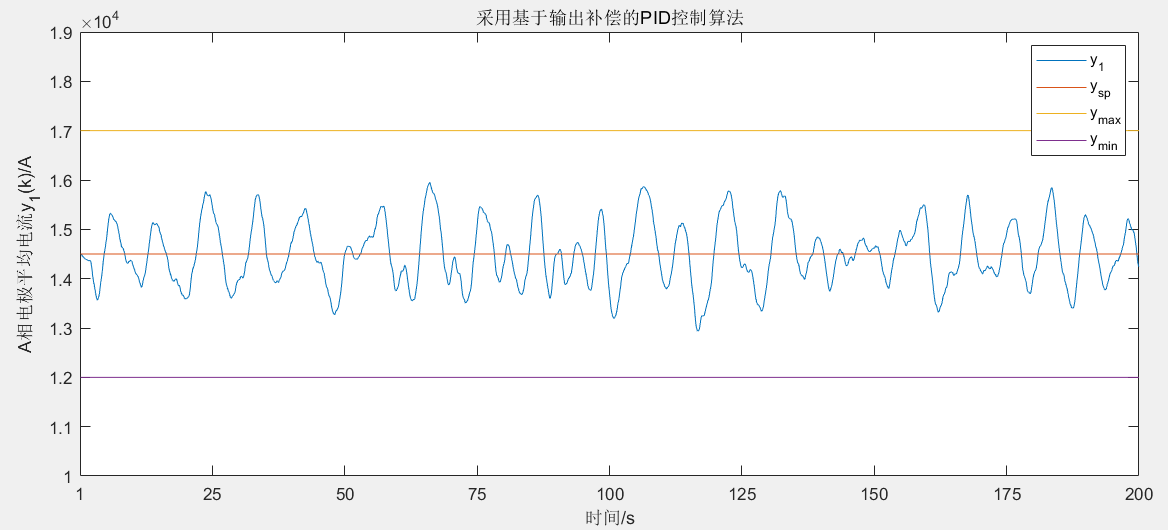
\includegraphics[width=.8\textwidth]{figure/输出补偿PID-输出信号.png} 
    \caption{使用基于输出补偿PID控制算法} % caption是图片的标题
    % \label{fig:img} % 此处的label相当于一个图片的专属标志,目的是方便上下文的引用
    % 图片引用格式:\ref{fig:img} 可能需要二次编译
\end{figure}
\begin{figure}[H]
    \centering % 居中 
    % 图片文件的相对路径
    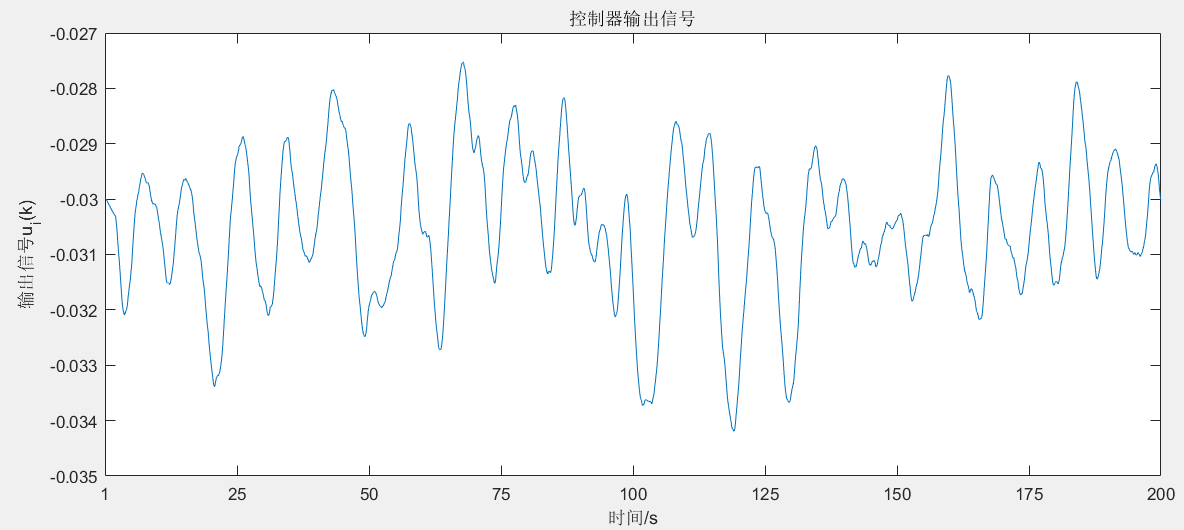
\includegraphics[width=.8\textwidth]{figure/输出补偿PID-控制信号.png} 
    \caption{使用基于输出补偿PID控制算法-控制信号输出} % caption是图片的标题
    % \label{fig:img} % 此处的label相当于一个图片的专属标志,目的是方便上下文的引用
    % 图片引用格式:\ref{fig:img} 可能需要二次编译
\end{figure}
\begin{figure}[H]
    \centering % 居中 
    % 图片文件的相对路径
    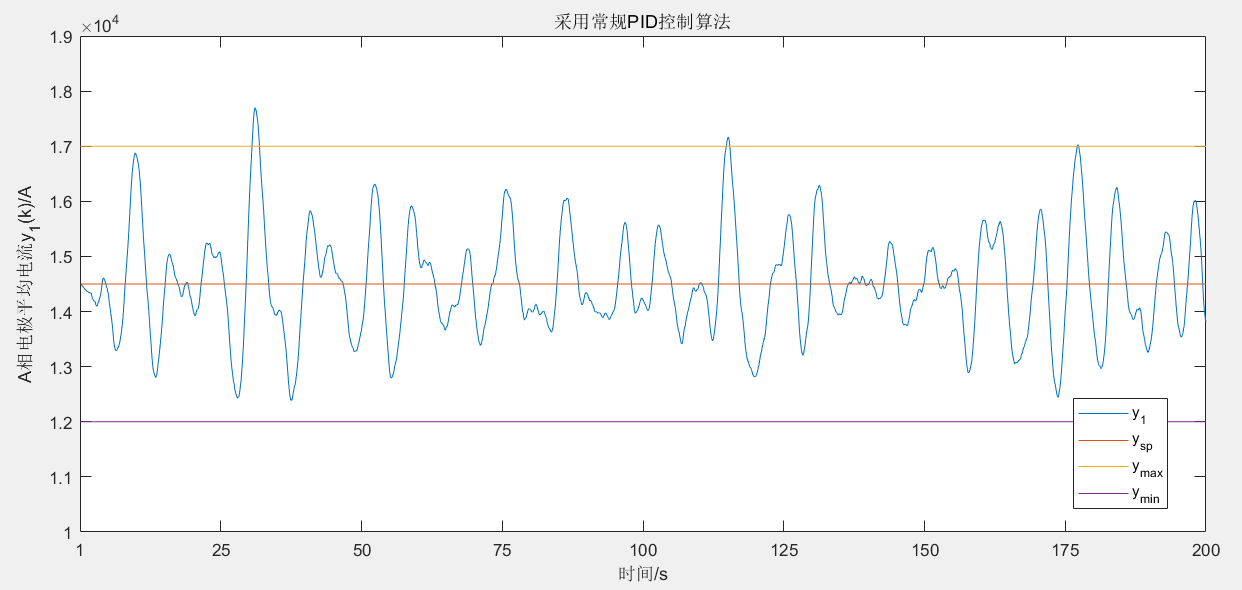
\includegraphics[width=.8\textwidth]{figure/常规PID-输出信号.png} 
    \caption{使用常规PID算法} % caption是图片的标题
    % \label{fig:img} % 此处的label相当于一个图片的专属标志,目的是方便上下文的引用
    % 图片引用格式:\ref{fig:img} 可能需要二次编译
\end{figure}
\begin{figure}[H]
    \centering % 居中 
    % 图片文件的相对路径
    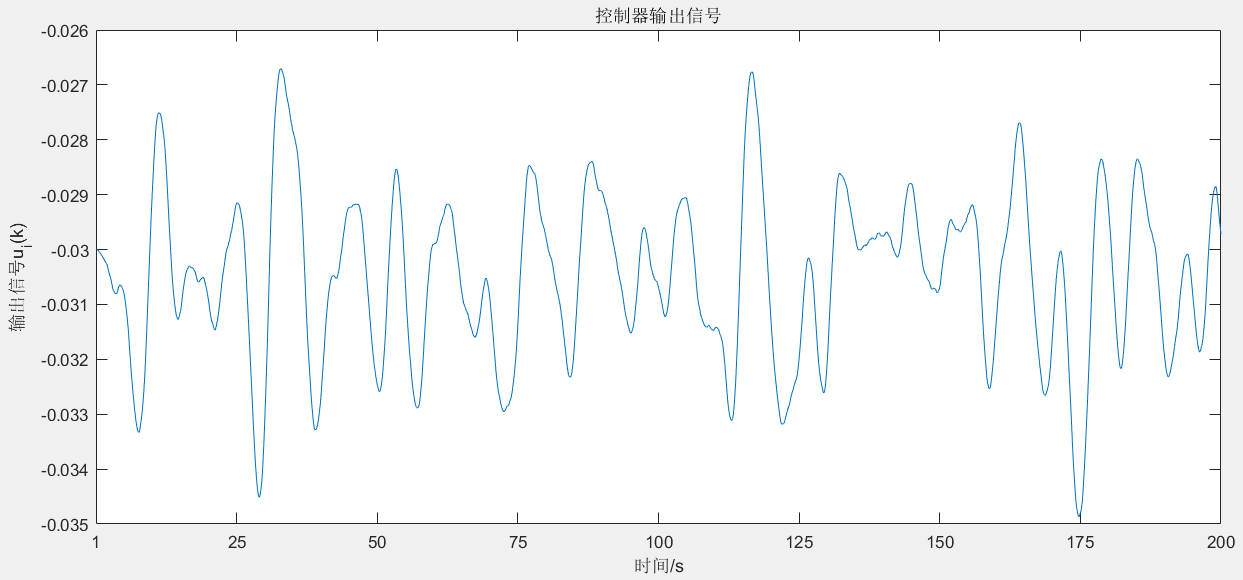
\includegraphics[width=.8\textwidth]{figure/常规PID-控制信号.png} 
    \caption{使用常规PID算法-控制信号输出} % caption是图片的标题
    % \label{fig:img} % 此处的label相当于一个图片的专属标志,目的是方便上下文的引用
    % 图片引用格式:\ref{fig:img} 可能需要二次编译
\end{figure}

由以上仿真实验结果可以看出,两种PID控制策略都可以将电极电流控制在设定值附近,且控制器输出到电机的控制信号都比较稳定,未出现超出限制范围的情况。在采用常规PID算法对电极电流进行控制时,电流的波动幅度较大,其跟踪误差绝对值有时会出现超出误差所允许最大上限值的情况;而使用文中所提出的基于输出补偿的PID控制算法时,可以明显地看出电流的波动幅度大幅减小,且在仿真实验的所有时间内均未出现跟踪误差超出上限值的情况,说明该方法更能满足实际的工艺要求。

% - 指标计算

%%
\subsection{基于补偿控制的自适应MPC算法的仿真验证}
%%%
\subsubsection{被控对象仿真模型与参数设定}
通过以上工艺流程分析可以知道,电熔镁砂熔炼过程以交流电机的转动方向和频率作为输入,以三相电极电流作为系统输出。此处作者为了方便后续处理,选取了三相电极中A相的电流作为系统输出,以得到一个单输入单输出的系统。最后得到的电熔镁砂熔炼过程中电机电流离散化的模型如下所示:
\begin{equation*}
	y(k+1) = y(k) + ay^2(k) + by^2(k)u(k) + \Delta y(k) + d_r(k)
\end{equation*}

其中,$y(k)$为$k$时刻的电极电流,$u(k)$为$k$时刻的电机转动方向和频率,$\Delta y(k)$为建模补偿误差;参数$a = \frac{\sqrt{3}}{\pi}\hat{F},\ b = -2\sqrt{3}\hat{Q}$,此处由于被控对象的特性,$\hat{F},\ \hat{Q}$代表的非线性函数随时间变化缓慢,因此将它们假设为常数,并入到待辨识的参数$a,\ b$当中。$d_r(k)$为系统受到的外部干扰,在仿真中人为设置成:
\begin{equation*}
	d_r(k) = 1000\sin(k\pi/20) + 1000\cos(k\pi/15)
\end{equation*}

结合具体的工艺过程,将电极电流的设定值设置为$y^*(k) = 15300A$,并且电极电流$y(k)$和电机的转动方向和频率的约束如下:
\begin{equation*}
	12000 < y(k) < 17000
\end{equation*}
\begin{equation*}
	-20 < u(k) < 20
\end{equation*}

此外,选择高阶观测器阶次$\eta = 2$;常值系数$L_0 = 0.8411,\ L_1 = 0.996,\ L_2 = 1$;参数估计向量初值$\hat{\theta}(0) = [-0.0024,\ -0.000074,\ 1]^T$;预测时域、控制时域$N_p = N_c = 4$;加权系数$s = 0.2,\ r = 0.1$;干扰观测器所需观测精度$D = 12$;参数估计精度$\gamma = \beta = 0.00000005$。此外,对于其中涉及到的MPC优化问题,这里使用MATLAB软件中自带的粒子群优化函数particleswarm()来解决。

%%%
\subsubsection{仿真结果}
基于以上设定,得到的仿真实验结果如下。

实验中使用的外部干扰信号$d_r(k)$如下图所示:
\begin{figure}[H]
    \centering % 居中 
    % 图片文件的相对路径
    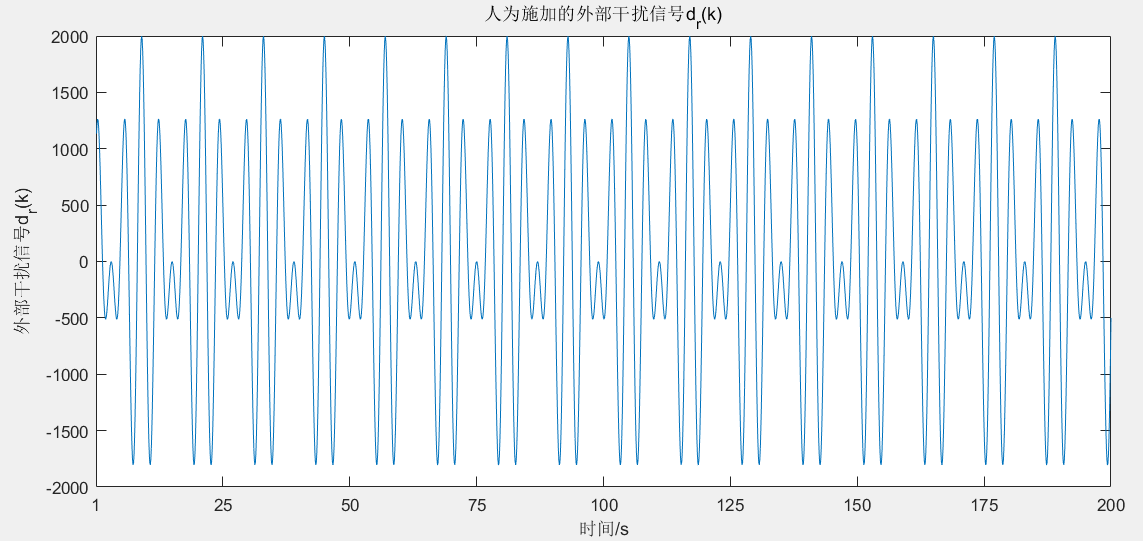
\includegraphics[width=.8\textwidth]{figure/模型预测-外部干扰信号.png} 
    \caption{外部干扰信号} % caption是图片的标题
    % \label{fig:img} % 此处的label相当于一个图片的专属标志,目的是方便上下文的引用
    % 图片引用格式:\ref{fig:img} 可能需要二次编译
\end{figure}

在电极电流设定值固定为$y_{sp}(k) = 15300A$时,A相电机电流控制结果以及控制器输出如下图所示:
\begin{figure}[H]
    \centering % 居中 
    % 图片文件的相对路径
    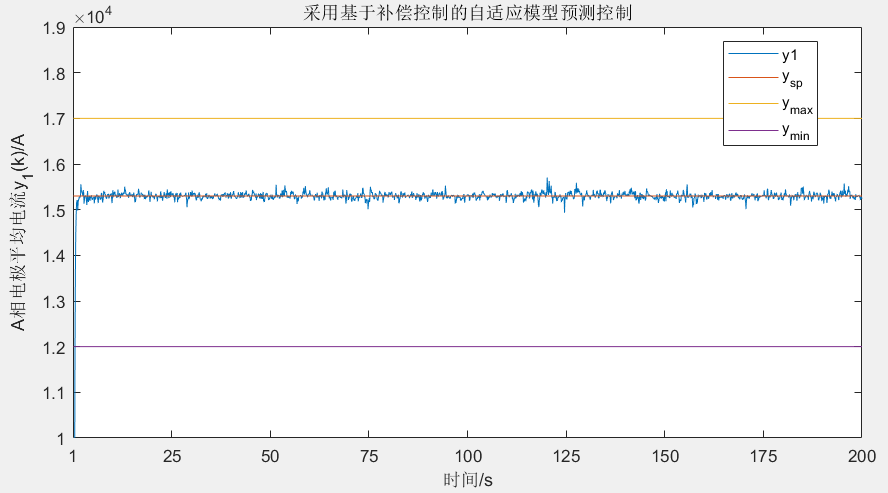
\includegraphics[width=.8\textwidth]{figure/模型预测-阶跃信号结果.png} 
    \caption{采用基于补偿控制的自适应模型预测控制方法的A相电极电流} % caption是图片的标题
    % \label{fig:img} % 此处的label相当于一个图片的专属标志,目的是方便上下文的引用
    % 图片引用格式:\ref{fig:img} 可能需要二次编译
\end{figure}
\begin{figure}[H]
    \centering % 居中 
    % 图片文件的相对路径
    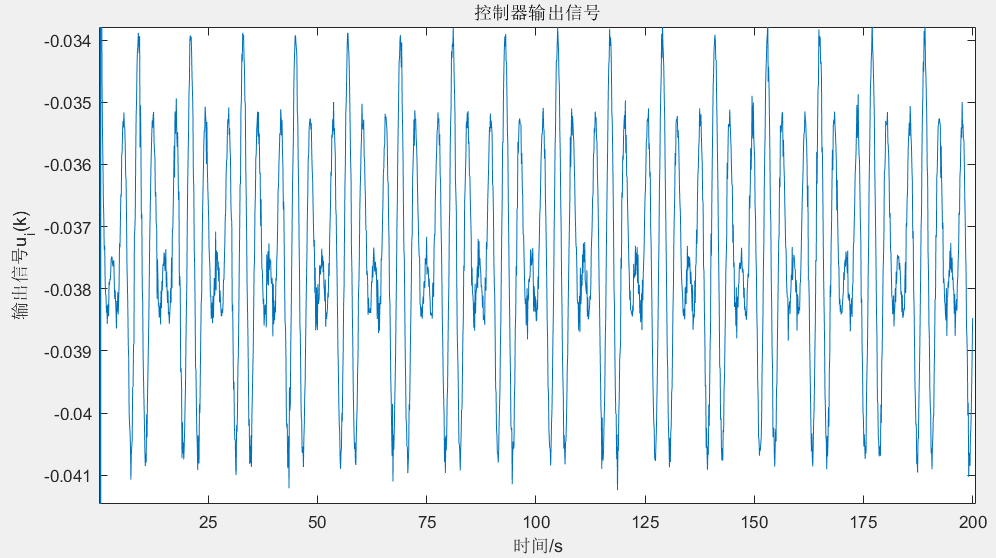
\includegraphics[width=.8\textwidth]{figure/模型预测-控制器输出信号-阶跃.png} 
    \caption{控制器输出信号} % caption是图片的标题
    % \label{fig:img} % 此处的label相当于一个图片的专属标志,目的是方便上下文的引用
    % 图片引用格式:\ref{fig:img} 可能需要二次编译
\end{figure}

当电极电流设定值在约束范围内突然出现变化时,A相电极电流的跟踪效果如下所示:
\begin{figure}[H]
    \centering % 居中 
    % 图片文件的相对路径
    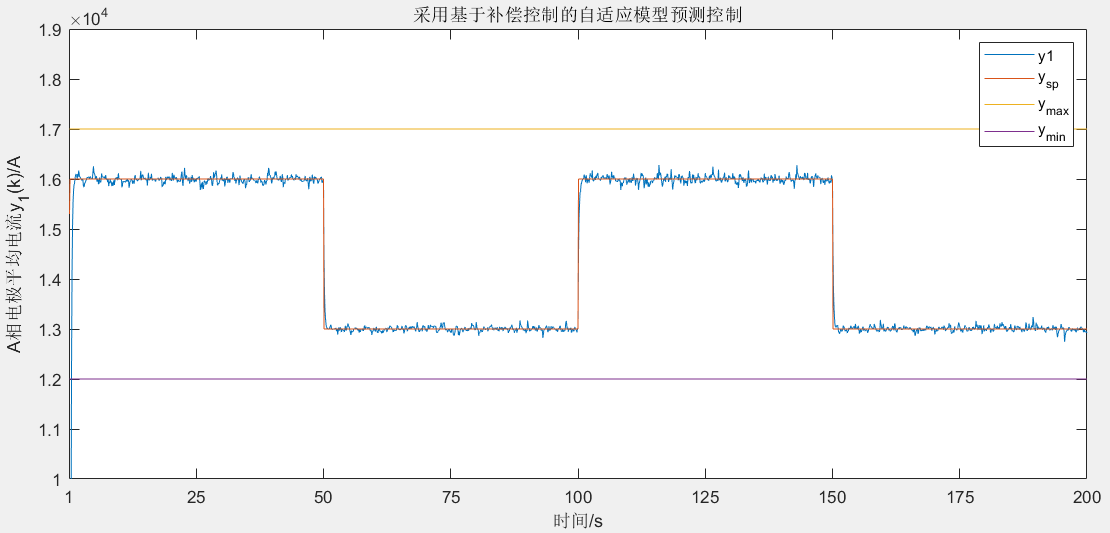
\includegraphics[width=.8\textwidth]{figure/模型预测-输出信号.png} 
    \caption{A相电极电流的跟踪效果} % caption是图片的标题
    % \label{fig:img} % 此处的label相当于一个图片的专属标志,目的是方便上下文的引用
    % 图片引用格式:\ref{fig:img} 可能需要二次编译
\end{figure}
\begin{figure}[H]
    \centering % 居中 
    % 图片文件的相对路径
    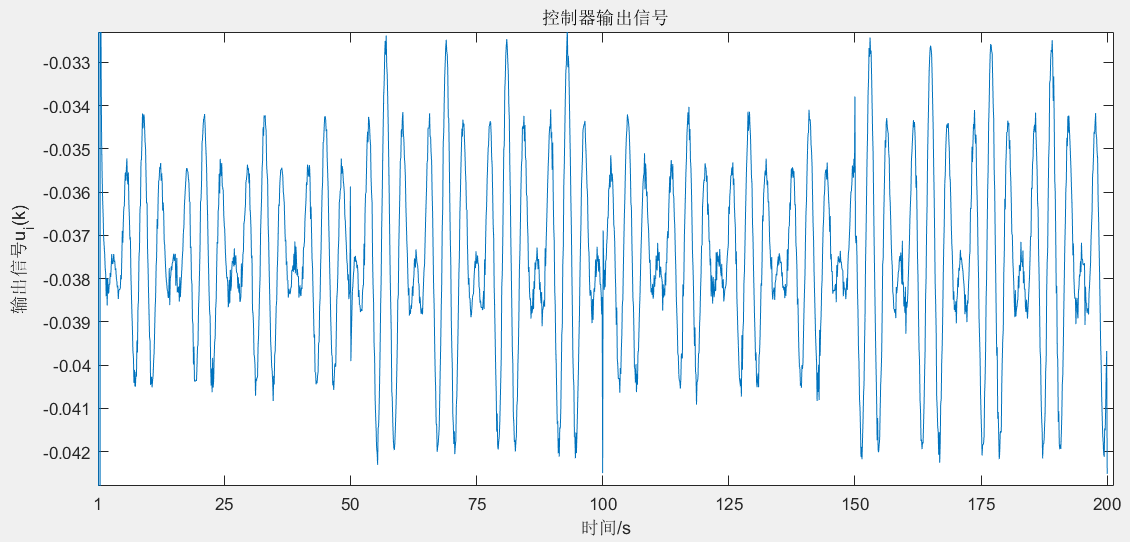
\includegraphics[width=.8\textwidth]{figure/模型预测-控制器输出信号.png} 
    \caption{控制器输出信号} % caption是图片的标题
    % \label{fig:img} % 此处的label相当于一个图片的专属标志,目的是方便上下文的引用
    % 图片引用格式:\ref{fig:img} 可能需要二次编译
\end{figure}

由以上仿真实验结果可以看出,基于补偿控制的自适应模型预测控制的控制效果相比前述带输出补偿的PID控制方法有了更大的提升,不仅电极电流波动的幅值更小,而且可以做到对不断变化的设定值进行实时跟踪。此外,相比论文中的实验结果,此处呈现的复现效果稍差,电极电流仍会出现一些毛刺状的波动,且电机的控制信号波动也稍显频繁,这些问题还有待进一步探究和解决。

%
\section{改进}

% - 可能存在的问题

在对熔炼过程电极电流动态模型进行建模时容易看出,电熔镁砂熔炼过程具有明显的强非线性。该论文在针对电极电流进行仿真实验时,对模型中的非线性函数,如$f_1(\cdot),\ f_2(\cdot),\ h_{ipool}(\cdot),\ \hat{h}_{ipool}(\cdot)$等进行了一些简化处理,并将它们近似看做常数。在文中介绍的具体实验过程中,针对这些常数首先需要使用实际工业过程中大量的电极电流和电机转动方向和频率数据,采用递推最小二乘和神经网络交替辨识方法对电流模型的参数进行预先辨识,然后将辨识得到的参数施加在模型中。这种处理方法存在一个问题,即模型中的上述非线性函数大多和原矿的性质如颗粒长度和杂质成分,以及熔炼过程的某些状态量有关。这些因素在实际工业生产过程中不可能是一成不变的,也就意味着在实际的熔炼过程中系统的参数在不断变化。因此,可以考虑在目前的控制方法基础上加入对系统主要参数的辨识算法,通过在线辨识的方式对模型不断更新和修正,个人认为这样可以提高控制系统对外界环境变化的自适应能力。

% 熔炼过程

% - 改进方式

% 附录 原论文
% 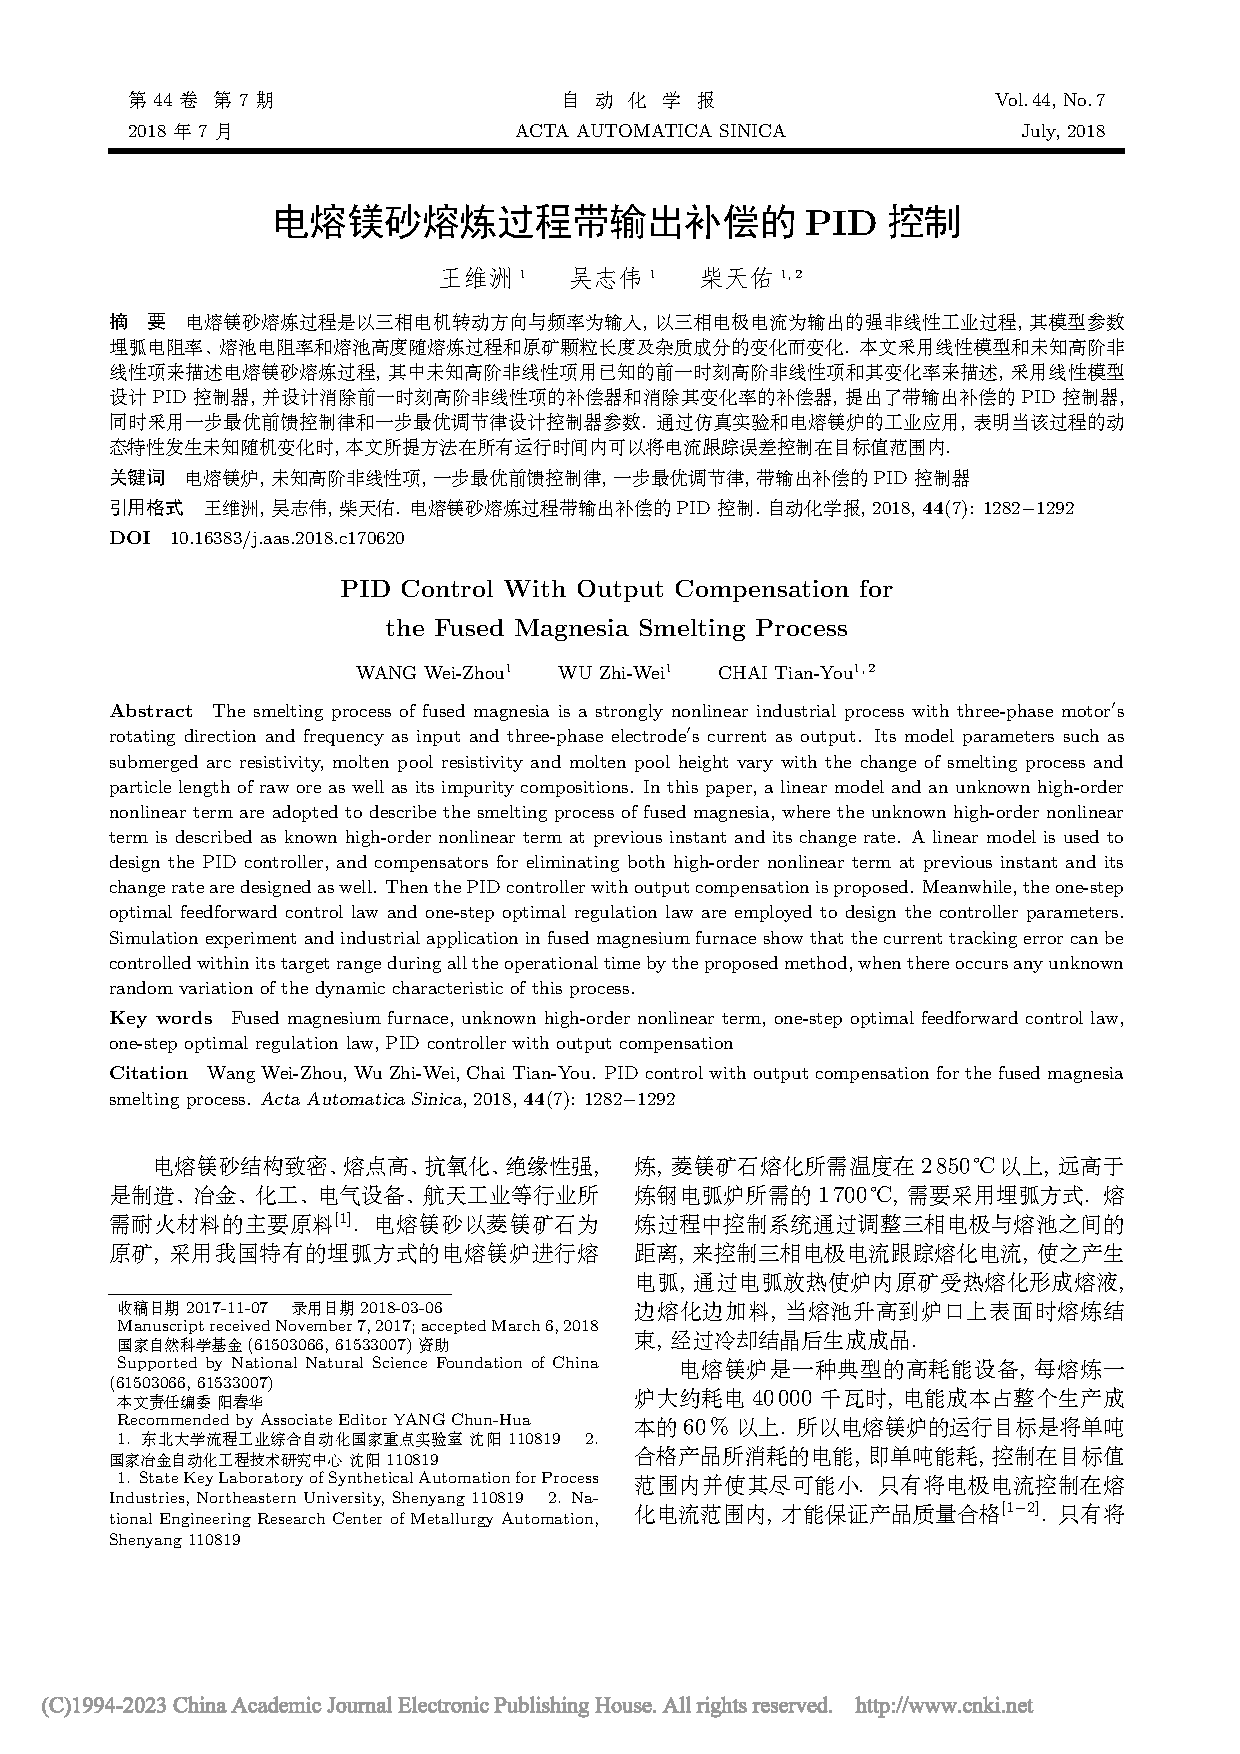
\includepdf[pages={1}]{./cover/file.pdf}

% 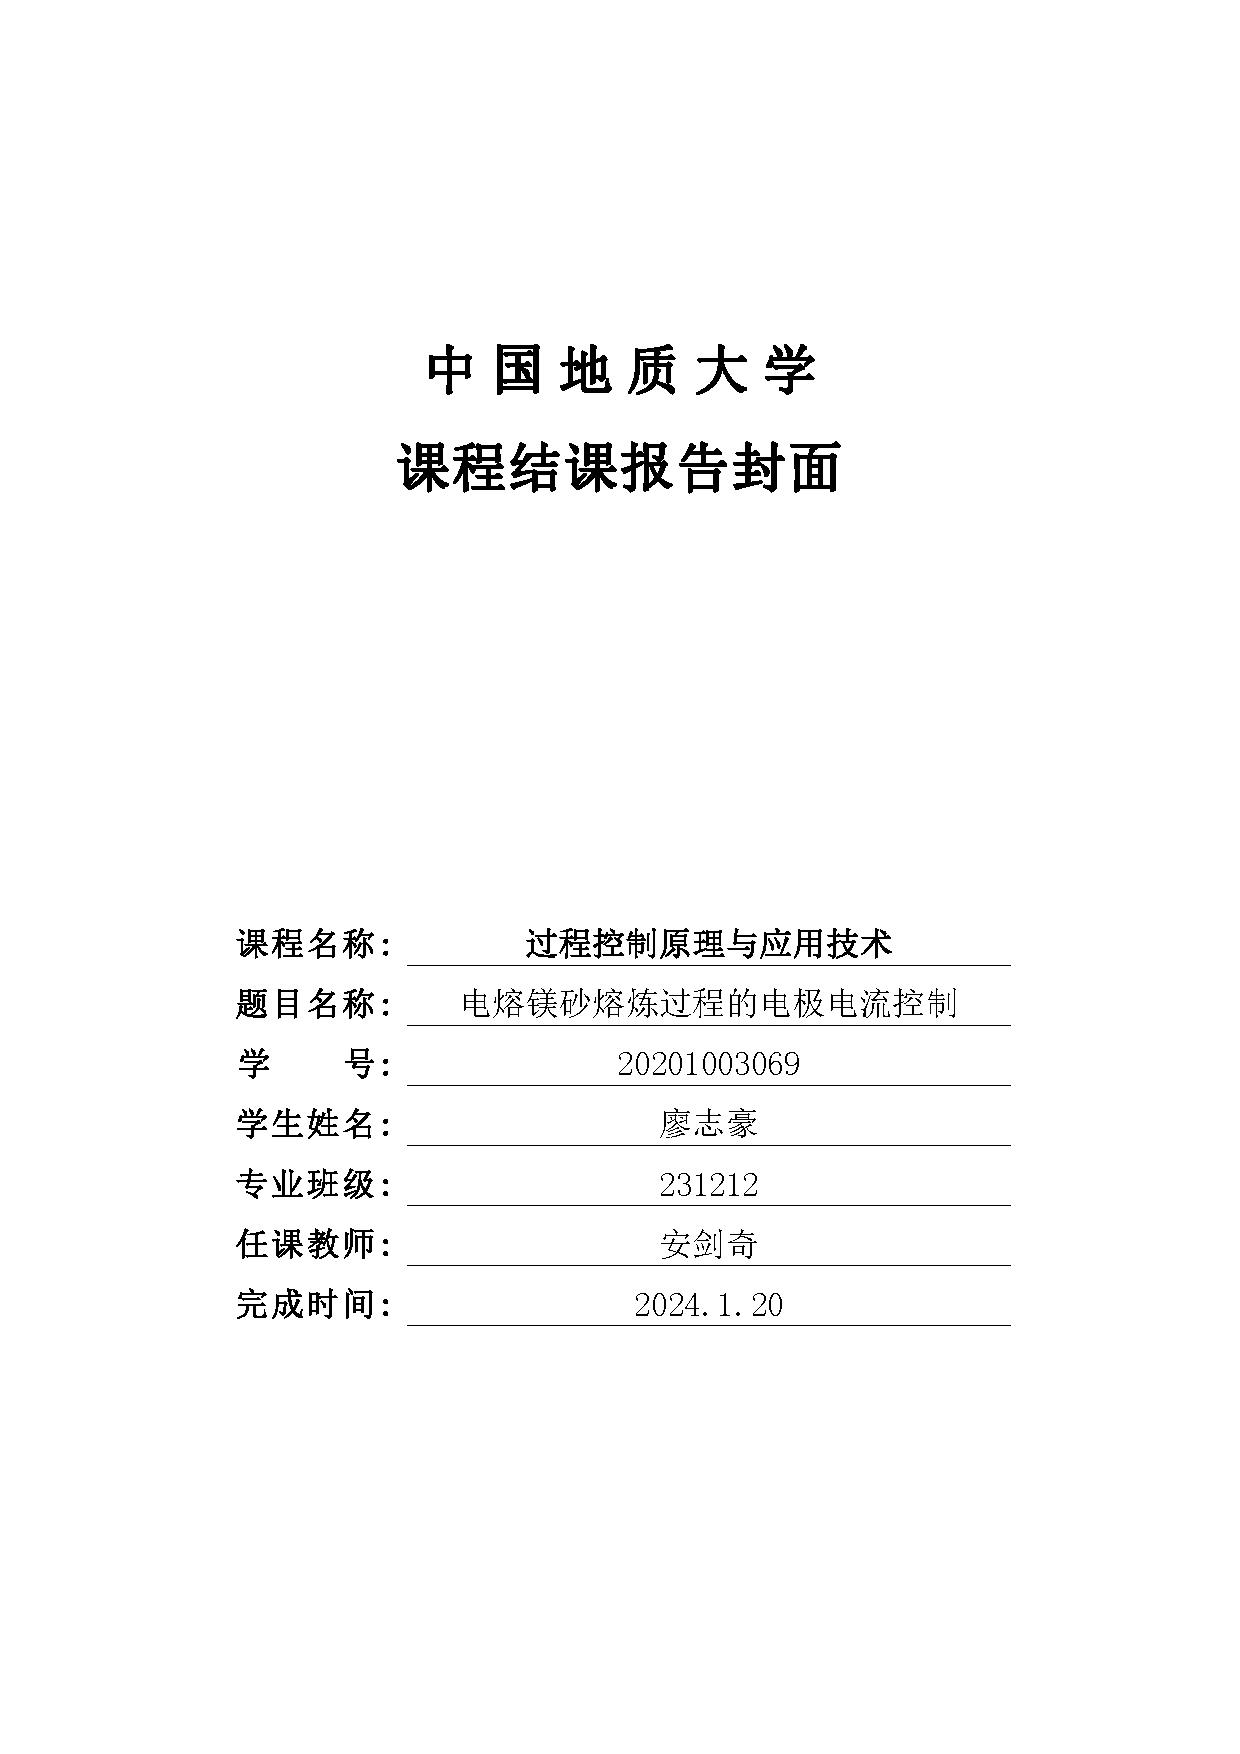
\includepdf[pages={1}]{./cover/cover.pdf}

\end{document}